\section{Experiments}
\label{sec:experiments}

\subsection{Experimental Setup}
\label{sec:setup}

\paragraph{TheAgentCompany.}
Our primary controlled study uses TheAgentCompany
\citep{theagentcompany}, which contains 127 workplace tasks and 542
execution-based checkpoints across GitLab, RocketChat, OwnCloud, and Plane.
Its six professional domains share tools, APIs, and workflows, providing
recurring procedural structure across tasks. The isolated services form a
resettable testbed for state-changing workplace actions. To model recurring
enterprise automation in which agents repeatedly encounter the same workflows,
training and test sets contain the same 127 tasks. We enforced strict post-consolidation guardrails to prevent case-specific data leakage. Each condition scores one
fresh attempt per task under the current memory store.

\paragraph{$\tau^2$-Bench Retail.}
We additionally use the retail domain of $\tau^2$-Bench
\citep{tau2bench} to examine in-domain generalization across disjoint train and
test sets. We define a custom operating procedure that is absent from the agent
harness and encode its requirements in the ground-truth action checkpoints. The
disjoint train and test tasks share substantial procedural knowledge through
common policy rules and tool workflows. The resulting benchmark contains 74
training tasks with 391 checkpoints and 40 test tasks with 192 checkpoints. Agents first execute the training
tasks without access to the procedure. The resulting traces and checkpoint
feedback are then used to construct each memory condition's store, which is
frozen and evaluated on the test tasks while the original procedure remains
withheld. 

\paragraph{Models, harnesses, and environments.}
For both benchmarks, we report results with Claude Opus 4.6 \citep{claudeopus46}, GPT-5.4 \citep{gpt54}, and
GLM-5 \citep{glm5}. On TheAgentCompany, we use the \texttt{pi-agent}
harness, which exposes bash as its only action tool for issuing API calls
against self-hosted services in isolated Docker environments. Cohere Embed v4
provides 1024-dimensional embeddings for semantic search. For $\tau^2$-Bench,
we use its native function-calling agent and simulated customer environment.
All memory methods receive the same training rollout batch, and LLM-based
methods use the same consolidator model
(Appendix~\ref{app:reproducibility}).

\paragraph{Metrics and controls.}
Our primary metric is \emph{checkpoint pass rate}: the fraction of binary,
execution-grounded checkpoints passed. For $\tau^2$-Bench, checkpoints are
ground-truth action sequences verified against the environment state.
\emph{Fully-passed rate} is the fraction of tasks satisfying all benchmark
evaluation criteria. We also report memory-store size and consolidation API
cost. The full four-dimensional controlled study is conducted on
TheAgentCompany, while $\tau^2$-Bench repeats the consolidation-method
comparison under held-out in-domain generalization.
Appendix~\ref{app:results} gives the complete matrix and exact results, and
Appendix~\ref{app:reproducibility} reports implementation details and costs.

\subsection{Consolidation Method}
\label{sec:exp1}

\begin{table}[tb]
\caption{\textbf{Consolidation method across model variants.}
Bold marks the best value for each metric within a block, and the shaded
row is the Free Form \method.}
\label{tab:exp1}
\centering
\small
\resizebox{\textwidth}{!}{
\begin{tabular}{l ccc ccc}
\toprule
& \multicolumn{3}{c}{\textsc{TheAgentCompany}} & \multicolumn{3}{c}{$\tau^2$\textsc{-Bench}} \\
\cmidrule(lr){2-4} \cmidrule(lr){5-7}
Method & Checkpoint pass & Fully passed & Store (KB) & Checkpoint pass & Fully passed & Store (KB) \\
\midrule
\rowcolor{ModelRow}
\multicolumn{7}{l}{\textbf{Claude Opus 4.6}} \\
No Memory          & 58.5\%                          & 36.2\%                          & n/a     & 66.7\%                          & 40.0\%                          & n/a     \\
No Consolidation   & 61.3\% {\scriptsize(+2.8)}      & 40.2\% {\scriptsize(+4.0)}      & 7{,}979 & 69.3\% {\scriptsize(+2.6)}      & 42.5\% {\scriptsize(+2.5)}      & 1{,}428 \\
SkillX             & 65.3\% {\scriptsize(+6.8)}      & 45.7\% {\scriptsize(+9.5)}      & 1{,}125 & \textbf{81.2\%} {\scriptsize(+14.5)} & 50.0\% {\scriptsize(+10.0)}     & 336     \\
Insights           & 65.7\% {\scriptsize(+7.2)}      & 45.7\% {\scriptsize(+9.5)}      & 396     & 78.1\% {\scriptsize(+11.4)}     & \textbf{55.0\%} {\scriptsize(+15.0)} & 96      \\
\cmidrule(lr){1-7}
\multicolumn{7}{l}{\textit{WASP-Mem}} \\
\rowcolor{OurRow}
\quad Free Form (Implicit Dedup)             & \textbf{72.3\%} {\scriptsize(+13.8)} & 48.0\% {\scriptsize(+11.8)}     & \textbf{234} & \textbf{81.2\%} {\scriptsize(+14.5)} & \textbf{55.0\%} {\scriptsize(+15.0)} & \textbf{92}  \\
\quad + Schema (Implicit Dedup)              & 66.2\% {\scriptsize(+7.7)}     & \textbf{48.8\%} {\scriptsize(+12.6)} & 565          & 77.6\% {\scriptsize(+10.9)}     & 42.5\% {\scriptsize(+2.5)}      & 252          \\
\quad + Schema + Explicit Dedup              & 65.7\% {\scriptsize(+7.2)}     & 44.9\% {\scriptsize(+8.7)}      & 789          & 79.7\% {\scriptsize(+13.0)}     & 52.5\% {\scriptsize(+12.5)}     & 656          \\
\midrule
\rowcolor{ModelRow}
\multicolumn{7}{l}{\textbf{GPT-5.4}} \\
No Memory          & 60.0\%                          & 40.2\%                          & n/a     & 65.1\%                          & 35.0\%                          & n/a     \\
No Consolidation   & 62.5\% {\scriptsize(+2.5)}      & 42.5\% {\scriptsize(+2.3)}      & 8{,}208 & 62.0\% {\scriptsize($-$3.1)}    & 42.5\% {\scriptsize(+7.5)}      & 1{,}953 \\
SkillX             & 67.2\% {\scriptsize(+7.2)}      & 50.4\% {\scriptsize(+10.2)}     & 1{,}161 & 69.3\% {\scriptsize(+4.2)}      & 45.0\% {\scriptsize(+10.0)}     & 425     \\
Insights           & 66.2\% {\scriptsize(+6.2)}      & 48.8\% {\scriptsize(+8.6)}      & 399     & 67.7\% {\scriptsize(+2.6)}      & 52.5\% {\scriptsize(+17.5)}     & \textbf{112} \\
\cmidrule(lr){1-7}
\multicolumn{7}{l}{\textit{WASP-Mem}} \\
\rowcolor{OurRow}
\quad Free Form (Implicit Dedup)             & \textbf{72.5\%} {\scriptsize(+12.5)} & \textbf{52.0\%} {\scriptsize(+11.8)} & \textbf{233} & \textbf{76.6\%} {\scriptsize(+11.5)} & \textbf{60.0\%} {\scriptsize(+25.0)} & 123          \\
\quad + Schema (Implicit Dedup)              & 67.9\% {\scriptsize(+7.9)}     & 50.4\% {\scriptsize(+10.2)}     & 592          & 71.4\% {\scriptsize(+6.3)}      & 47.5\% {\scriptsize(+12.5)}     & 303          \\
\quad + Schema + Explicit Dedup              & 67.0\% {\scriptsize(+7.0)}     & 49.6\% {\scriptsize(+9.4)}      & 808          & 71.9\% {\scriptsize(+6.8)}      & 52.5\% {\scriptsize(+17.5)}     & 880          \\
\midrule
\rowcolor{ModelRow}
\multicolumn{7}{l}{\textbf{GLM-5}} \\
No Memory          & 58.9\%                          & 38.6\%                          & n/a     & 47.4\%                          & 25.0\%                          & n/a     \\
No Consolidation   & 61.8\% {\scriptsize(+2.9)}      & 40.9\% {\scriptsize(+2.3)}      & 8{,}480 & 46.4\% {\scriptsize($-$1.0)}    & 30.0\% {\scriptsize(+5.0)}      & 1{,}461 \\
SkillX             & 65.7\% {\scriptsize(+6.8)}      & 46.5\% {\scriptsize(+7.9)}      & 1{,}187 & 53.1\% {\scriptsize(+5.7)}      & 32.5\% {\scriptsize(+7.5)}      & 315     \\
Insights           & 65.9\% {\scriptsize(+7.0)}      & 47.2\% {\scriptsize(+8.6)}      & 441     & 51.6\% {\scriptsize(+4.2)}      & 37.5\% {\scriptsize(+12.5)}     & \textbf{82}  \\
\cmidrule(lr){1-7}
\multicolumn{7}{l}{\textit{WASP-Mem}} \\
\rowcolor{OurRow}
\quad Free Form (Implicit Dedup)             & \textbf{72.5\%} {\scriptsize(+13.6)} & \textbf{52.0\%} {\scriptsize(+13.4)} & \textbf{255} & \textbf{58.3\%} {\scriptsize(+10.9)} & \textbf{42.5\%} {\scriptsize(+17.5)} & 92           \\
\quad + Schema (Implicit Dedup)              & 66.6\% {\scriptsize(+7.7)}     & 50.4\% {\scriptsize(+11.8)}     & 599          & 56.2\% {\scriptsize(+8.8)}      & 37.5\% {\scriptsize(+12.5)}     & 323          \\
\quad + Schema + Explicit Dedup              & 65.7\% {\scriptsize(+6.8)}     & 46.5\% {\scriptsize(+7.9)}      & 838          & 53.1\% {\scriptsize(+5.7)}      & 27.5\% {\scriptsize(+2.5)}      & 557          \\
\bottomrule
\end{tabular}}
\end{table}

\subsubsection{Main Results}
\label{sec:exp1-main-results}

This experiment tests whether consolidating experience improves future execution
and how the organization of procedural memory affects transfer. We compare No
Memory, raw-trace retrieval without consolidation, Insights, SkillX, and the
three \method{} variants. All conditions use checkpoint-binary feedback,
ingest both successful and failed traces, and consolidate in a single round
(R1). Within each benchmark, all memory methods receive the same training
rollout batch and are evaluated under the same execution budget.


Table~\ref{tab:exp1} shows that consolidation, rather than experience storage
alone, drives improvement. Every consolidated method exceeds No Memory across
all six model--benchmark combinations. In contrast, No Consolidation provides
only +2.5--2.9 pp on TheAgentCompany and changes checkpoint pass rate by
$-3.1$ to +2.6 pp on $\tau^2$-Bench. Raw traces can therefore preserve useful
examples, but without abstraction and reconciliation they transfer
inconsistently and can even distract execution.

Free Form \method{} provides the strongest and most consistent result. It leads
checkpoint pass rate for every model on TheAgentCompany and leads or ties the
best baseline on $\tau^2$-Bench (tying SkillX for Claude at 81.2\%), improving
by +10.9--14.5 pp over No Memory across the six settings. It also improves
fully-passed rate by +11.8--25.0 pp and achieves the best or tied-best value
in five of six settings. These gains do not come from retaining more
experience: its 92--255 KB stores are approximately 94--97\% smaller than No
Consolidation. Free Form is the smallest consolidated store for all three
TheAgentCompany models and the smallest \method{} variant on $\tau^2$-Bench.

The \method{} ablations further show that prescriptive knowledge organization
does not improve consolidation. Adding a human-defined schema lowers checkpoint
pass rate relative to Free Form in every model--benchmark combination by
2.1--6.1 pp, while increasing store size by 2.3--3.5$\times$. Adding explicit
deduplication also remains 1.5--6.8 pp below Free Form and expands the store by
3.3--7.2$\times$. Thus, agent-managed implicit deduplication produces a more
compact and effective procedural memory than either prescribed page types or
prescribed cross-session matching rules.

Figure~\ref{fig:filter-size} reinforces that a compact memory store with high signal density outperforms a large one
filled with redundancy and noise. \emph{These results
suggest that memory consolidation acts as a filter. Its value lies not in
volume but in selectivity, retaining informative procedural signal while
discarding what is false, noisy, redundant, or misleading.} Under this view,
we identify two failure modes:

\begin{itemize}[leftmargin=*,itemsep=2pt,topsep=3pt]
    \item \textbf{Under-filtering} retains noise, redundancy, and incidental
    detail. No Consolidation stores entire rollouts without abstraction.
    Insights and SkillX abstract individual sessions but process them
    independently, so similar procedures with nuanced differences produce
    separate entries rather than being merged into a shared, deduplicated
    procedure.
    \item \textbf{Over-filtering} discards useful signal. Schema Form's fixed
    fields can exclude implementation details not anticipated when the schema
    was designed. SkillX's rigid three-level hierarchy may similarly drop
    contextual information that does not fit its prescribed structure.
\end{itemize}

\noindent
These two modes can co-occur: a method may simultaneously retain redundant
entries (under-filtering) while discarding actionable detail that falls outside
its prescribed structure (over-filtering), producing a mis-filtered store.
Free Form \method{} achieves a more balanced filter: reading the existing wiki
before writing enables implicit deduplication, while unconstrained pages
preserve whichever actionable details execution reveals, yielding the strongest
and most consistent checkpoint pass rate across model variants.

\begin{promptwrapper}{Let Agents Organize Memory.}
\textbf{Prescriptive knowledge organization does not improve consolidation. Agent management produces more compact and effective procedural memory.}
\end{promptwrapper}


\subsection{Feedback Type and Ingestion Scope}
\label{sec:exp23}

This experiment asks how feedback richness and trace-ingestion scope jointly
affect consolidation quality. It uses Free Form \method{} consolidated in a
single round (R1). Feedback varies from \emph{Self-Judge}, to external
\emph{Checkpoint-binary} outcomes, to \emph{Checkpoint-binary + Human}
feedback with natural-language diagnosis. Within each feedback condition, we
compare \emph{Success-only} ingestion with \emph{Both}, which also admits
failed traces. The two scopes consolidate the same R0 rollout batch and
receive the same subsequent execution budget, so their difference isolates the
value of learning from failure.

\begin{figure}[tb]
\centering
\begin{subfigure}[t]{0.43\linewidth}
    \centering
    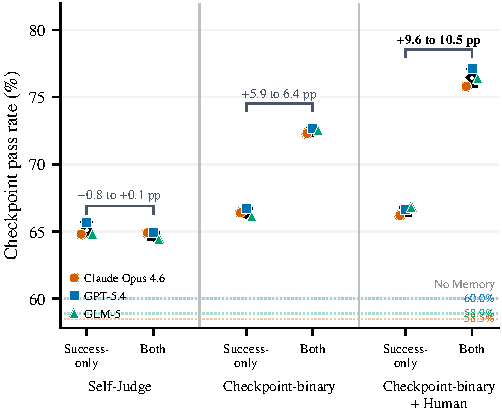
\includegraphics[width=\linewidth]{fig_ingestion_scope_checkpoint.pdf}
    \caption{Checkpoint pass rate.}
    \label{fig:ingestion-scope-checkpoint}
\end{subfigure}\hfill
\begin{subfigure}[t]{0.43\linewidth}
    \centering
    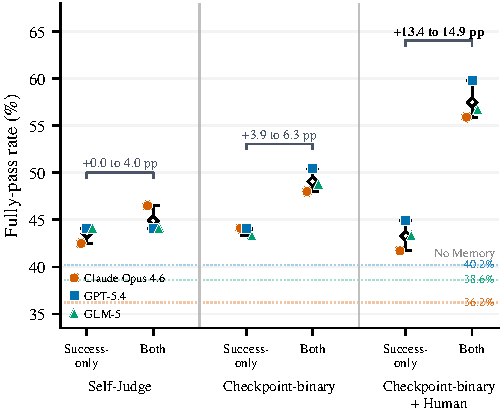
\includegraphics[width=\linewidth]{fig_ingestion_scope_fullpass.pdf}
    \caption{Full pass rate.}
    \label{fig:ingestion-scope-full}
\end{subfigure}
\caption{\textbf{Feedback type and ingestion scope.}
Checkpoint pass rate (a) and fully-passed rate (b) when consolidating
successful traces only versus both successful and failed traces under
Self-Judge, Checkpoint-binary, and Checkpoint-binary + Human feedback.
Colored points denote model variants; black diamonds and whiskers show the
cross-model mean and min--max range.}
\label{fig:feedback-scope}
\end{figure}

Feedback richness first determines the overall quality of the consolidated
memory. When both successful and failed traces are ingested, checkpoint pass
rate rises from 64.4--64.9\% with Self-Judge to 72.3--72.7\% with
Checkpoint-binary and 75.8--77.1\% with Checkpoint-binary + Human. External
checkpoint outcomes improve performance by +7.4--8.1 pp over Self-Judge by
correcting mistaken self-assessments and localizing unsuccessful actions.
Human diagnosis adds a further +3.5--4.4 pp by explaining failure causes and
corrective procedures that cannot be recovered reliably from a binary outcome
alone.

This benefit is concentrated in failed traces. Under Success-only ingestion,
moving from Self-Judge to Checkpoint-binary + Human changes checkpoint pass
rate by only +0.9--2.0 pp, and adding human diagnosis beyond Checkpoint-binary
changes it by $-0.2$ to +0.7 pp. Under Both, the same comparisons yield
+10.9--12.2 pp and +3.5--4.4 pp, respectively. Fully-passed rate exhibits the
same interaction: rich feedback changes Success-only by only $-0.8$ to
+0.8 pp over Self-Judge, but improves Both by +9.4--15.7 pp. Diagnostic
feedback therefore contributes primarily by making failed executions
interpretable, rather than by adding substantial information to traces that
already succeeded.

Viewed from the other axis, richer feedback determines how much the agent can
learn from failed traces (Figure~\ref{fig:feedback-scope}). Moving from
Success-only to Both changes checkpoint pass rate by only $-0.7$ to +0.1 pp
under Self-Judge. Without reliable external signal, the agent cannot
distinguish a reusable lesson from incidental unsuccessful behavior, so
admitting failures adds noise rather than knowledge. The gain grows to
+5.9--6.4 pp with Checkpoint-binary feedback and +9.6--10.5 pp with
Checkpoint-binary + Human feedback. The fully-passed rate exhibits the same
progression: admitting failed traces adds 0.0--4.0 pp under Self-Judge,
+3.9--6.3 pp under Checkpoint-binary, and +13.4--14.9 pp under
Checkpoint-binary + Human. Failure traces are therefore not automatically
useful: they become valuable when feedback identifies what failed and, most
effectively, why it failed and how the procedure should be corrected.

\begin{promptwrapper}{Feedback Makes Failure Learnable.}
\textbf{The richer and more diagnostic the feedback, the more downstream value
the agent extracts from failed traces.}
\end{promptwrapper}


\subsection{Multi-Round Refinement}
\label{sec:multi-round}

This experiment asks whether repeated execution and consolidation continue to
close the residual procedural-knowledge gap. It uses Free Form \method{} with
Both ingestion scope, varies rounds from R0 through R4, and compares
Self-Judge, Checkpoint-binary, and Checkpoint-binary + Human feedback. R0
executes without memory; each subsequent round executes against the current
frozen store and then consolidates the resulting traces and feedback. All
reported results reflect fresh executions from that round rather than
cumulative or best-over-round scores.

\begin{figure}[tb]
\centering
\begin{subfigure}[t]{0.43\linewidth}
    \centering
    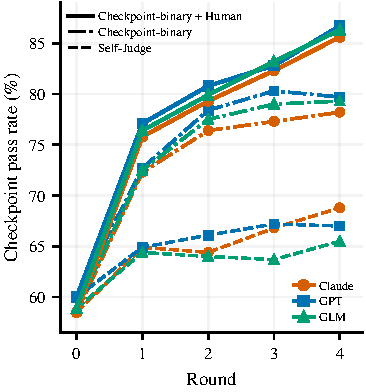
\includegraphics[width=\linewidth]{fig_rounds_refinement.pdf}
    \caption{Reactive refinement.}
    \label{fig:rounds-refinement}
\end{subfigure}\hfill
\begin{subfigure}[t]{0.5\linewidth}
    \centering
    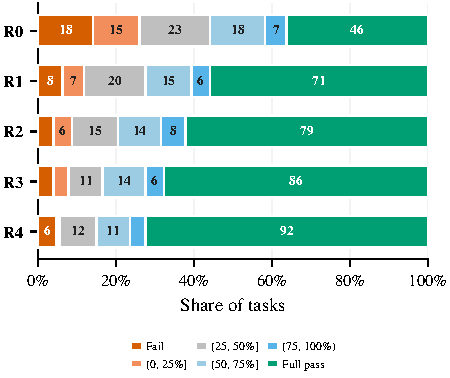
\includegraphics[width=\linewidth]{fig_task_completion.pdf}
    \caption{Progress toward full pass.}
    \label{fig:rounds-completion}
\end{subfigure}
\caption{\textbf{Multi-round refinement and task completion.}
(a) Checkpoint pass rate across R0--R4 for all three models under
Checkpoint-binary + Human, Checkpoint-binary, and Self-Judge feedback.
(b) Claude Opus 4.6 task scores under Checkpoint-binary + Human feedback.
Segment labels are task counts.}
\label{fig:rounds}
\end{figure}

With Checkpoint-binary + Human feedback, checkpoint pass rate increases
monotonically for every model and reaches 85.6--86.7\% at R4. The first
consolidation round contributes +17.1--17.5 pp, yet the residual failures
continue to reveal useful procedural gaps: R3 to R4 still adds +3.1--3.9 pp,
with gains remaining non-trivial through the final round. Checkpoint-binary
feedback reaches only 78.2--79.7\% at R4, with its final-round change
shrinking to $-0.6$ to +0.9 pp. Self-Judge is lower and non-monotonic, ending
at 65.5--68.8\%. Human diagnosis therefore does more than improve the first
memory store; it repeatedly turns the remaining failures into new corrective
knowledge.

Feedback quality also matters more than additional rounds alone. After one
Checkpoint-binary + Human round, checkpoint pass rate is already
75.8--77.1\%, exceeding the corresponding Self-Judge R4 result by
7.0--10.9 pp for every model. Four rounds of self-assessment do not recover
the information supplied by one round of external outcomes and human failure
diagnosis.

Figure~\ref{fig:rounds-completion} shows how local checkpoint gains translate
into end-to-end task success. For Claude Opus 4.6, fully passed tasks increase
from 46 at R0 to 71, 79, 86, and 92 through R4. As repeated refinement makes
earlier steps reliable and resolves later failure points, tasks shift from
partial completion into full passes.

\begin{promptwrapper}{Feedback Quality over Rollout Volume.}
\textbf{Richer feedback on fewer traces outperforms sparse feedback on more
rollouts; local checkpoint gains compound into end-to-end success.}
\end{promptwrapper}

